Introduction to threads and how to use them

\par
\par
\par
\hypertarget{threads_threads_intro}{}\subsection{Intro}\label{threads_threads_intro}
A thread, also called a thread of execution is the smallest sequence of program instructions that can be managed by an operating system scheduler. Multi-\/threading is implemented by time-\/division multiplexing where the processor switches between threads. Context switching occurs fast enough that the user perceives the threads as running at the same time. By using threads a programmer can split the work into the threads, each responsible for a smaller portion of the problem. From a threads view he thinks it has the processor all to itself.\hypertarget{threads_kern_threads}{}\subsubsection{e\-Solid R\-T Kernel thread}\label{threads_kern_threads}
e\-Solid R\-T Kernel supports multi-\/threading and allows applications to have any number of threads. The only limiting factors for the maximum number of threads are the amount of R\-A\-M and R\-O\-M memory and processing time.

Threads are implemented as normal {\ttfamily C} functions. Thread functions must have the following prototype\-:


\begin{DoxyCode}
\textcolor{keywordtype}{void} fn (\textcolor{keywordtype}{void} *);
\end{DoxyCode}


Which in plain english means\-: {\itshape fn is a function (pointer to void) returning void}.\hypertarget{threads_kern_threads_state}{}\subsubsection{Thread states}\label{threads_kern_threads_state}
A thread can be in one of the following states\-: \begin{center}

\begin{DoxyImageNoCaption}
  \mbox{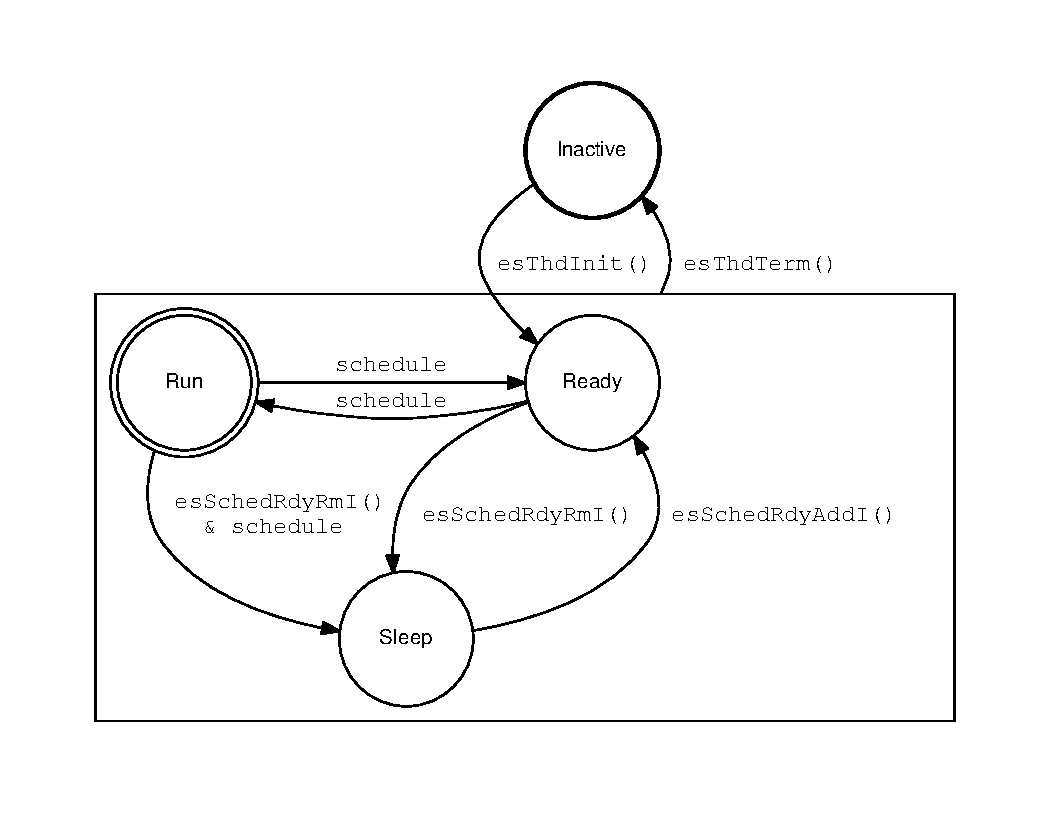
\includegraphics[width=\textwidth,height=\textheight/2,keepaspectratio=true]{dot_inline_dotgraph_2}}
\end{DoxyImageNoCaption}
\end{center}
 \begin{DoxyParagraph}{Inactive}
This is thread initial state. Threads in this state are still not activated ({\bfseries inactive}) by \hyperlink{group__kern__intf_gac91734f3ee867b519f59bf81cc7fde88}{es\-Thd\-Init()} function or they were deleted by \hyperlink{group__kern__intf_gac9d1eac76f26096614e8196bcfd8b905}{es\-Thd\-Term()} function. The scheduler does not recognize these threads and they will never execute.
\end{DoxyParagraph}
\begin{DoxyParagraph}{Ready}
Threads waiting to execute. There are the threads that are {\bfseries ready} to execute but are not currently executing because a different thread (equal or higher priority) is already executing.
\end{DoxyParagraph}
\begin{DoxyParagraph}{Run}
Thread is currently executing. When the thread is in this state then the code is actually being {\bfseries run} on the processor.
\end{DoxyParagraph}
\begin{DoxyParagraph}{Sleep}
Thread is sleeping. These threads are {\bfseries sleeping} while waiting for an event to occur.
\end{DoxyParagraph}
\hypertarget{threads_thd_create}{}\subsection{Initializing Threads}\label{threads_thd_create}
\hypertarget{threads_thd_create_init}{}\subsubsection{es\-Thd\-Init() A\-P\-I function}\label{threads_thd_create_init}
Threads are initialized by using \hyperlink{group__kern__intf_gac91734f3ee867b519f59bf81cc7fde88}{es\-Thd\-Init()} A\-P\-I function.

\begin{DoxyParagraph}{Stack size}

\end{DoxyParagraph}
There is no easy way to determine the stack size required by a thread. It is possible to calculate approximate stack size for simple threads, but for more complex ones (e.\-g. which calls library A\-P\-I function) this can be a daunting task. In this case stack size will be set to a size more than adequate for the thread and then use the profiling features provided by the kernel to ensure both that the space allocated is adequate, and that R\-A\-M space is not being unnecessarily wasted. 